\chapter{CW-复形}
\begin{introduction}
    \item 本节介绍了一类好的拓扑空间---CW 复形, 粗略来说, 它是通过不断将 $n$ 维圆盘 $\mathbb{D}^n$ 沿着其边界 $\mathbb{S}^{n-1}$ 粘接到空间上所构成的空间(因此具有自然的维数定义).
    \item CW 复形是一类足够好的空间, 它具有很强的一般性: 例如, 每个拓扑空间都同伦等价于某个 CW 复形(该定理称为 CW 逼近), 并且在 CW 复形中弱同伦等价即为同伦等价.
    \item 从 CW 复形出发可以定义出与奇异同调等价的胞腔同调理论.
    \item 从同伦代数的角度来看, CW 复形是是 Quillen 模型结构中的双纤维性对象(因此其实可以将 CW 逼近视为余纤维性替换, 这将在第~\ref{抽象同伦论}~章中提到).
\end{introduction}
\section{定义}
回忆到 $\mathbb{S}^n \hookrightarrow \mathbb{D}^n$ 为满足同伦延拓性质的余纤维化, 其中 $\mathbb{D}^n$ 为 $n$ 维\textbf{圆盘}且 
$S^{n-1} = \partial \mathbb{D}^n$ 为其边界, 即 $(n-1)$ 维球面.令
\[
    e^n = (\mathbb{D}^n)^{\circ} = \mathbb{D}^n - \partial \mathbb{D}^n
\]
表示 $\mathbb{D}^n$ 的内部, 该开圆盘称为 $n$ 维\textbf{胞腔}.\\
CW-复形所构成的范畴由可以被 $n$ 维胞腔(像乐高一样, 具体由 $S^{n-1} \hookrightarrow \mathbb{D}^n$) 所构建的拓扑空间所组成.
此外, 它具有很强的一般性\footnote{在英文原文中所述的是:``Moreover, it is large enough to cover most interesting examples.''}.
\begin{definition}
    空间 $X$ 的\textbf{胞腔分解}为一族 $X$ 的子空间
    \[
        \mathcal{E} = \{e_{\alpha}^n | \alpha \in J_n\}
    \]
    使得每个 $e_{\alpha}^n$ 均为 $n$维胞腔且有集合的无交并
    \[
        X = \coprod e_{\alpha}^n.
    \]
    $X$ 的 $n$维\textbf{骨架}为子空间
    \[
        X^n = \coprod_{\alpha \in J_m , m\leq n} e_{\alpha}^n.
    \]
\end{definition}
\begin{definition}
    CW 复形是指由 Hausdorff 空间以及其胞腔分解所构成的二元组 $(X,\mathcal{E})$, 使得
    \begin{enumerate}
        \item 特征映射: 对于每个 $n$ 维胞腔都有一个特征映射
        \[
            \Phi_{e_{\alpha}^n} \colon \mathbb{D}^n \to X
        \]
        使得其限制在 $(\mathbb{D}^n)^{\circ}$ 上同胚于 $e_{\alpha}^n$ 且 $\Phi_{e_{\alpha}^n}(S^{n-1}) \subset X^{n-1}$.
        \item \textbf{C = 闭包有限性:} 对于任意胞腔 $e\in \cal{E}$ 其闭包 $\bar{e}$ 只与有限个 $\cal{E}$ 中的胞腔相交.
        \item \textbf{W = 弱拓扑:} 考虑子集 $A \subset X$, 它是闭的当且仅当对于每个 $e\in \cal{E}$ 都有 $A\cap \bar{e}$ 在 $\bar{e}$ 中闭.
    \end{enumerate} 
    称 $X$ 为 $n$ 维 CW-复形, 指 $\cal{E}$ 中胞腔的维数最大为 $n$ 的 CW 复形.
\end{definition}
注意到 $X$ 的 Hausdorff 性质说明对于每个胞腔 $e\in \cal{E}$ 都有 $\bar{e} = \Phi_e(\mathbb{D}^n)$. 
满射 $\Phi_e \colon \mathbb{D}^n \to \bar{e}$ 为商映射是因为 $\mathbb{D}^n$ 为紧空间且 $\bar{e}$ 是 Hausdorff 的.
记全体特征映射为
\[
    \Phi : \coprod_{e\in \mathcal{E}}\mathbb{D}^n \xrightarrow{\coprod \Phi_e} X.
\]    
由弱拓扑推知 $\Phi$ 是商映射. 由此推出以下命题.
\begin{proposition}
    令 $(X,\mathcal{E})$ 为 CW 复形. 则 $f\colon X \to Y$ 连续当且仅当
    \[
        f\circ \Phi_e \colon \mathbb{D}^n \to Y
    \]
    对于每个 $e\in \cal{E}$ 都是连续的.
\end{proposition}
\begin{proposition}
    令 $(X,\mathcal{C})$ 为 CW 复形. 则任意 $X$ 的紧子空间都只与有限多个胞腔有交.
\end{proposition}
\begin{proof}
    不妨设存在 $X$ 的紧子空间 $K$ 使其与无限多个胞腔有交. 令 $x_i \in K\cap e_i$, $i=1,2,\cdots$, 
    其中 $e_i$ 为不同的胞腔. 考虑子集
    \[
        Z_m = \{x_m,x_{m+1},\cdots\}, \quad m\geq 1.
    \]
    根据闭包有限性, 可知 $Z_m$ 与每个闭包 $\bar{e}$ 至多交于有限个点, 因此根据 Hausdorff 性可知其在 $\bar{e}$ 中是闭的.
    由弱拓扑可知, $Z_m$ 为 $X$ 的闭子集, 因此在 $K$ 中闭. 观察到
    \[
        \bigcap_{m \geq 1} Z_m = \varnothing
    \]
    但是 $Z_m$ 的任意有限交都是非空的, 这与 $K$ 的紧性相矛盾.
\end{proof}
\begin{proposition}
    令 $(X,\mathcal{E})$ 为 CW 复形且 $X^n$ 为 $n$ 维骨架. 则 $X$ 为以下(望远镜)图表的余极限(即正向极限)
    \[
        X^1 \to X^2 \to \cdots \to X^n \to \cdots
    \]
\end{proposition}
\begin{proof}
    由弱拓扑的泛性质可知 $f\colon X \to Y$ 连续当且仅当 $f\mid_{X^n} \colon X^n \to Y$ 对于每个 $n$ 都连续.
\end{proof}
\begin{proposition}
    令 $(X,\mathcal{E})$ 为 CW 复形. 则 $X$ 为紧生成弱 Hausdorff 空间.
\end{proposition}
\begin{proof}
    $X$ 为 Hausdorff 故自然弱 Hausdorff, 接下来说明 $X$ 为紧生成空间.\\
    令 $Z \subset X$ 为 k-闭子空间, 因每个胞腔的闭包 $\bar{e}$ 都是紧 Hausdorff 的, $Z\cap \bar{e}$ 在 $\bar{e}$ 中闭.\\
    弱拓扑推知 $Z$ 在 $X$ 中闭, 因此 $kX = X$.
\end{proof}
\begin{example}
    以下是一些经典示例.
    \begin{itemize}
        \item $n$ 维球面可以分解为 $0$ 维胞腔以及 $n$ 维胞腔
        \[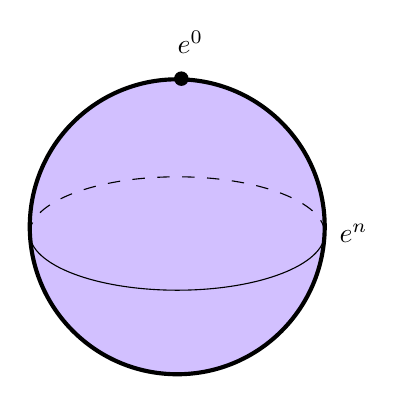
\begin{tikzpicture}[x=0.75pt,y=0.75pt,yscale=-1,xscale=1]
        \draw  [fill={rgb, 255:red, 210; green, 192; blue, 255 }  ,fill opacity=1 ][line width=1.5]  (217,132.06) .. controls (217,92.81) and (248.81,61) .. (288.06,61) .. controls (327.3,61) and (359.11,92.81) .. (359.11,132.06) .. controls (359.11,171.3) and (327.3,203.11) .. (288.06,203.11) .. controls (248.81,203.11) and (217,171.3) .. (217,132.06) -- cycle ; 
        \draw  [draw opacity=0][dash pattern={on 4.5pt off 4.5pt}] (217.01,135.79) .. controls (217,135.63) and (217,135.46) .. (217,135.3) .. controls (217,120.21) and (248.81,107.98) .. (288.06,107.98) .. controls (327.3,107.98) and (359.11,120.21) .. (359.11,135.3) .. controls (359.11,135.65) and (359.09,136) .. (359.06,136.35) -- (288.06,135.3) -- cycle ; \draw  [dash pattern={on 4.5pt off 4.5pt}] (217.01,135.79) .. controls (217,135.63) and (217,135.46) .. (217,135.3) .. controls (217,120.21) and (248.81,107.98) .. (288.06,107.98) .. controls (327.3,107.98) and (359.11,120.21) .. (359.11,135.3) .. controls (359.11,135.65) and (359.09,136) .. (359.06,136.35) ;  
        \draw  [draw opacity=0] (359.1,134.8) .. controls (359.11,134.97) and (359.11,135.13) .. (359.11,135.3) .. controls (359.11,150.39) and (327.3,162.62) .. (288.06,162.62) .. controls (248.81,162.62) and (217,150.39) .. (217,135.3) .. controls (217,134.94) and (217.02,134.59) .. (217.05,134.24) -- (288.06,135.3) -- cycle ; \draw   (359.1,134.8) .. controls (359.11,134.97) and (359.11,135.13) .. (359.11,135.3) .. controls (359.11,150.39) and (327.3,162.62) .. (288.06,162.62) .. controls (248.81,162.62) and (217,150.39) .. (217,135.3) .. controls (217,134.94) and (217.02,134.59) .. (217.05,134.24) ;  
        \draw  [color={rgb, 255:red, 0; green, 0; blue, 0 }  ,draw opacity=1 ][line width=5.25] [line join = round][line cap = round] (290.04,60.69) .. controls (290.04,60.69) and (290.04,60.69) .. (290.04,60.69) ;
        \draw (365,129.4) node [anchor=north west][inner sep=0.75pt]    {$e^{n}$};
        \draw (287,36.4) node [anchor=north west][inner sep=0.75pt]    {$e^{0}$};
        \end{tikzpicture}\]
        此时, 有
        \[
            \mathbb{S}^n = e^0 \cup e^n
        \]
        \item $n$ 维球面可以视为两个 $n$ 维胞腔以及一个 $n-1$ 维球面:
        \[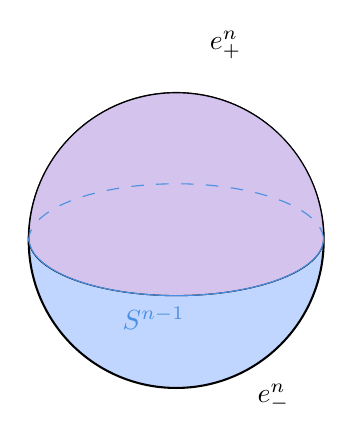
\begin{tikzpicture}[x=0.75pt,y=0.75pt,yscale=-1,xscale=1]
        \draw  [fill={rgb, 255:red, 192; green, 214; blue, 255 }  ,fill opacity=1 ][line width=0.75]  (216.97,134.66) .. controls (216.97,95.41) and (248.78,63.6) .. (288.03,63.6) .. controls (327.27,63.6) and (359.08,95.41) .. (359.08,134.66) .. controls (359.08,173.9) and (327.27,205.71) .. (288.03,205.71) .. controls (248.78,205.71) and (216.97,173.9) .. (216.97,134.66) -- cycle ;
        \draw  [color={rgb, 255:red, 0; green, 0; blue, 0 }  ,draw opacity=1 ][fill={rgb, 255:red, 211; green, 195; blue, 237 }  ,fill opacity=1 ] (288.06,161.23) .. controls (248.84,161.23) and (217.06,149) .. (217.06,133.91) -- (217.03,133.91) .. controls (217.03,95.02) and (248.83,63.5) .. (288.06,63.5) .. controls (327.28,63.5) and (359.08,95.02) .. (359.08,133.91) -- (359.05,133.91) .. controls (359.05,149) and (327.27,161.23) .. (288.06,161.23) -- cycle ;
        \draw  [draw opacity=0][dash pattern={on 4.5pt off 4.5pt}] (216.98,135.15) .. controls (216.97,134.99) and (216.97,134.82) .. (216.97,134.66) .. controls (216.97,119.57) and (248.78,107.34) .. (288.03,107.34) .. controls (327.27,107.34) and (359.08,119.57) .. (359.08,134.66) .. controls (359.08,135.01) and (359.06,135.36) .. (359.03,135.71) -- (288.03,134.66) -- cycle ; \draw  [color={rgb, 255:red, 74; green, 144; blue, 226 }  ,draw opacity=1 ][dash pattern={on 4.5pt off 4.5pt}] (216.98,135.15) .. controls (216.97,134.99) and (216.97,134.82) .. (216.97,134.66) .. controls (216.97,119.57) and (248.78,107.34) .. (288.03,107.34) .. controls (327.27,107.34) and (359.08,119.57) .. (359.08,134.66) .. controls (359.08,135.01) and (359.06,135.36) .. (359.03,135.71) ;  
        \draw  [draw opacity=0] (359.11,133.53) .. controls (359.11,133.53) and (359.11,133.53) .. (359.11,133.53) .. controls (359.11,148.83) and (327.31,161.23) .. (288.08,161.23) .. controls (248.86,161.23) and (217.06,148.83) .. (217.06,133.53) .. controls (217.06,133.53) and (217.06,133.53) .. (217.06,133.53) -- (288.08,133.53) -- cycle ; \draw  [color={rgb, 255:red, 74; green, 144; blue, 226 }  ,draw opacity=1 ] (359.11,133.53) .. controls (359.11,133.53) and (359.11,133.53) .. (359.11,133.53) .. controls (359.11,148.83) and (327.31,161.23) .. (288.08,161.23) .. controls (248.86,161.23) and (217.06,148.83) .. (217.06,133.53) .. controls (217.06,133.53) and (217.06,133.53) .. (217.06,133.53) ;  
        \draw (303,32.4) node [anchor=north west][inner sep=0.75pt]    {$e_{+}^{n}$};
        \draw (261,165.4) node [anchor=north west][inner sep=0.75pt]  [color={rgb, 255:red, 74; green, 144; blue, 226 }  ,opacity=1 ]  {$S^{n-1}$};
        \draw (326,202.4) node [anchor=north west][inner sep=0.75pt]    {$e_{-}^{n}$};
        \end{tikzpicture}\]
        此时有
        \begin{align*}
            \mathbb{S}^n &= e_+^n \cup e_-^n \cup S^{n-1}\\
            &= \left(e_+^n\cup e_-^n\right)\cup\left( e_+^{n-1}\cup e_-^{n-1} \right)\cup \cdots \cup \left( e_+^0\cup e_-^0 \right)
        \end{align*}
        \item $\R^n$ 网格/立方体分解为 $n$-立方体 $I^n \simeq \mathbb{D}^n$.
        \[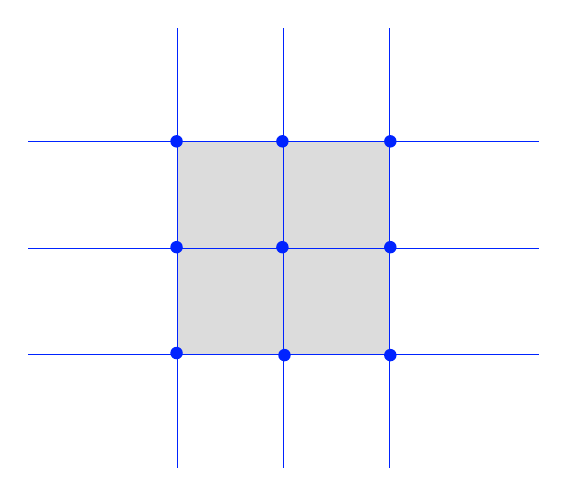
\begin{tikzpicture}[x=0.75pt,y=0.75pt,yscale=-1,xscale=1]
        \draw  [color={rgb, 255:red, 0; green, 35; blue, 255 }  ,draw opacity=1 ][fill={rgb, 255:red, 155; green, 155; blue, 155 }  ,fill opacity=0.35 ] (281.58,89.95) -- (332.83,89.95) -- (332.83,141.2) -- (281.58,141.2) -- cycle ;
        \draw  [color={rgb, 255:red, 0; green, 35; blue, 255 }  ,draw opacity=1 ][fill={rgb, 255:red, 155; green, 155; blue, 155 }  ,fill opacity=0.35 ] (281.58,141.2) -- (332.83,141.2) -- (332.83,192.44) -- (281.58,192.44) -- cycle ;
        \draw  [color={rgb, 255:red, 0; green, 35; blue, 255 }  ,draw opacity=1 ][fill={rgb, 255:red, 155; green, 155; blue, 155 }  ,fill opacity=0.35 ] (230.33,89.95) -- (281.58,89.95) -- (281.58,141.2) -- (230.33,141.2) -- cycle ;
        \draw  [color={rgb, 255:red, 0; green, 35; blue, 255 }  ,draw opacity=1 ][fill={rgb, 255:red, 155; green, 155; blue, 155 }  ,fill opacity=0.35 ] (230.33,141.2) -- (281.58,141.2) -- (281.58,192.44) -- (230.33,192.44) -- cycle ;
        \draw  [color={rgb, 255:red, 0; green, 35; blue, 255 }  ,draw opacity=1 ]   (158.58,89.95) -- (404.58,89.95) ;
        \draw  [color={rgb, 255:red, 0; green, 35; blue, 255 }  ,draw opacity=1 ]   (158.58,141.2) -- (404.58,141.2) ;
        \draw  [color={rgb, 255:red, 0; green, 35; blue, 255 }  ,draw opacity=1 ]   (158.58,192.44) -- (404.58,192.44) ;
        \draw  [color={rgb, 255:red, 0; green, 35; blue, 255 }  ,draw opacity=1 ]   (230.33,35.2) -- (230.33,247.2) ;
        \draw  [color={rgb, 255:red, 0; green, 35; blue, 255 }  ,draw opacity=1 ]   (281.58,35.2) -- (281.58,247.2) ;
        \draw  [color={rgb, 255:red, 0; green, 35; blue, 255 }  ,draw opacity=1 ]   (332.83,35.2) -- (332.83,247.2) ;
        \draw  [color={rgb, 255:red, 0; green, 35; blue, 255 }  ,draw opacity=1 ][line width=4.5] [line join = round][line cap = round] (230.04,191.69) .. controls (230.04,191.69) and (230.04,191.69) .. (230.04,191.69) ;
        \draw  [color={rgb, 255:red, 0; green, 35; blue, 255 }  ,draw opacity=1 ][line width=4.5] [line join = round][line cap = round] (230.04,140.69) .. controls (230.04,140.69) and (230.04,140.69) .. (230.04,140.69) ;
        \draw  [color={rgb, 255:red, 0; green, 35; blue, 255 }  ,draw opacity=1 ][line width=4.5] [line join = round][line cap = round] (230.04,89.69) .. controls (230.04,89.69) and (230.04,89.69) .. (230.04,89.69) ;
        \draw  [color={rgb, 255:red, 0; green, 35; blue, 255 }  ,draw opacity=1 ][line width=4.5] [line join = round][line cap = round] (281.04,89.69) .. controls (281.04,89.69) and (281.04,89.69) .. (281.04,89.69) ;
        \draw  [color={rgb, 255:red, 0; green, 35; blue, 255 }  ,draw opacity=1 ][line width=4.5] [line join = round][line cap = round] (281.04,140.69) .. controls (281.04,140.69) and (281.04,140.69) .. (281.04,140.69) ;
        \draw  [color={rgb, 255:red, 0; green, 35; blue, 255 }  ,draw opacity=1 ][line width=4.5] [line join = round][line cap = round] (282.04,192.69) .. controls (282.04,192.69) and (282.04,192.69) .. (282.04,192.69) ;
        \draw  [color={rgb, 255:red, 0; green, 35; blue, 255 }  ,draw opacity=1 ][line width=4.5] [line join = round][line cap = round] (333.04,89.69) .. controls (333.04,89.69) and (333.04,89.69) .. (333.04,89.69) ;
        \draw  [color={rgb, 255:red, 0; green, 35; blue, 255 }  ,draw opacity=1 ][line width=4.5] [line join = round][line cap = round] (333.04,140.69) .. controls (333.04,140.69) and (333.04,140.69) .. (333.04,140.69) ;
        \draw  [color={rgb, 255:red, 0; green, 35; blue, 255 }  ,draw opacity=1 ][line width=4.5] [line join = round][line cap = round] (333.04,192.69) .. controls (333.04,192.69) and (333.04,192.69) .. (333.04,192.69) ;
        \end{tikzpicture}\]
        \item $\mathbb{CP}^n \colon (\CC^{n+1}-\{0\})/\sim$ 并且有
        \[
            \mathbb{CP}^0\subset \mathbb{CP}^1 \subset \cdots \subset \mathbb{CP}^{n-1}\subset \cdots \subset \mathbb{CP}^{\infty}.
        \]
        此外,
        \begin{align*}
            \mathbb{CP}^n - \mathbb{CP}^{n-1} &= \{[z_0,\cdots,z_n]\colon z_n \neq 0\}\\
            &\simeq \CC^{n} \simeq e^{2n}.
        \end{align*}
        因此 $\mathbb{CP}^n$ 在 $0$ 到 $2n$ 的每个偶数维上都只有一个胞腔以及特征映射
        \begin{align*}
            \Phi_{2n} \colon D^{2n} &\to \mathbb{CP}^n\\
            (z_0,\cdots,z_n) &\mapsto \left[ z_0,\cdots, z_{n-1} \sqrt{1-\sum_{i=0}^{n-1} |z_i|^2} \right]
        \end{align*}
    \end{itemize}
\end{example}
\begin{definition}
    CW 复形 $(X,\mathcal{E})$ 的子复形 $(X',\mathcal{E}')$ 定义为闭子空间 $X'\subset X$ 以及胞腔分解 $\mathcal{E}'\subset \mathcal{E}$.
    在胞腔分解是自明的时候, 将其简写为 $X'\subset X$. 
    我们也记 $X' = |\mathcal{E}'|$. 等价的说, 子复形被描述为子集 $\mathcal{E}'\subset \mathcal{E}$ 使得
    \[
        e_1\in \mathcal{E}', e_2\in\mathcal{E}, \bar{e}_1\cap e_2 \neq \varnothing\Rightarrow e_2\in \mathcal{E}'.
    \] 
\end{definition}
\begin{example}
    $X$ 的 $n$ 维骨架 $X^n$ 就是维数 $\leq n$ 的子复形.
\end{example}
\subsection{粘接胞腔}
\begin{definition}
    给定 $f\colon S^{n-1} \to X$. 考虑推出
    \[\begin{tikzcd}
	{S^{n-1}} & X \\
	{\mathbb{D}^n} & {\mathbb{D}^n \coprod_f X}
	\arrow[from=1-1, to=1-2]
	\arrow[hook, from=1-1, to=2-1]
	\arrow[hook, from=1-2, to=2-2]
	\arrow["{\Phi_f}", from=2-1, to=2-2]
    \end{tikzcd}\]
    我们称 $\mathbb{D}^n \coprod_f X$ 为 $X$ 粘接上一个 $n$ 维胞腔. $\Phi_f$ 称为粘接 $n$ 维胞腔的特征映射. 

    更一般的, 若有一族映射 $f_{\alpha} \colon S^{n-1} \to X$, 令 $f = \coprod f_{\alpha}$, 则推出
    \[\begin{tikzcd}
	{\coprod_{\alpha}S^{n-1}} & X \\
	{\coprod_{\alpha}\mathbb{D}^n} & {\left(\coprod \mathbb{D}^n\right) \coprod_f X}
	\arrow["f", from=1-1, to=1-2]
	\arrow[hook, from=1-1, to=2-1]
	\arrow[hook, from=1-2, to=2-2]
	\arrow["{\Phi_f}", from=2-1, to=2-2]
    \end{tikzcd}\]
    称为往 $X$ 上粘接 $n$ 维胞腔.
\end{definition}
    \[\begin{tikzpicture}
\draw [color={rgb, 255:red, 0; green, 55; blue, 255 }  ,draw opacity=1 ][fill={rgb, 255:red, 184; green, 233; blue, 134 }  ,fill opacity=0.55 ]   (438.64,178) .. controls (528.64,179.44) and (527.34,109.88) .. (438.34,110.17) ;
%Shape: Arc [id:dp7271433133840051] 
\draw  [draw opacity=0][fill={rgb, 255:red, 184; green, 233; blue, 134 }  ,fill opacity=0.55 ] (306.65,179.27) .. controls (286.42,187.81) and (258.65,193.07) .. (228,193.07) .. controls (166.13,193.07) and (115.97,171.61) .. (115.97,145.14) .. controls (115.97,118.67) and (166.13,97.21) .. (228,97.21) .. controls (258.33,97.21) and (285.85,102.37) .. (306.02,110.75) -- (228,145.14) -- cycle ; \draw  [color={rgb, 255:red, 0; green, 55; blue, 255 }  ,draw opacity=1 ] (306.65,179.27) .. controls (286.42,187.81) and (258.65,193.07) .. (228,193.07) .. controls (166.13,193.07) and (115.97,171.61) .. (115.97,145.14) .. controls (115.97,118.67) and (166.13,97.21) .. (228,97.21) .. controls (258.33,97.21) and (285.85,102.37) .. (306.02,110.75) ;  
%Shape: Polygon [id:ds2902711184583131] 
\draw  [draw opacity=0][fill={rgb, 255:red, 184; green, 233; blue, 134 }  ,fill opacity=0.55 ] (306.02,110.75) -- (294.11,141.28) -- (306.65,179.27) -- (228,145.14) -- cycle ;
%Straight Lines [id:da23622301511185095] 
\draw    (308.02,112.75) -- (296.11,143.28) -- (308.65,181.27) ;
%Shape: Polygon [id:ds6853034016174555] 
\draw  [color={rgb, 255:red, 0; green, 55; blue, 255 }  ,draw opacity=1 ][fill={rgb, 255:red, 80; green, 227; blue, 194 }  ,fill opacity=1 ][line width=1.5]  (306.02,110.75) -- (329.11,123.28) -- (328.11,165.28) -- (306.65,179.27) -- (294.11,141.28) -- cycle ;
%Curve Lines [id:da5755177974699757] 
\draw [color={rgb, 255:red, 0; green, 55; blue, 255 }  ,draw opacity=1 ][fill={rgb, 255:red, 255; green, 255; blue, 255 }  ,fill opacity=1 ]   (193,145.14) .. controls (204.11,131.51) and (242.11,130.51) .. (263,145.14) ;
%Curve Lines [id:da5103795382625878] 
\draw [color={rgb, 255:red, 0; green, 120; blue, 255 }  ,draw opacity=1 ][fill={rgb, 255:red, 255; green, 255; blue, 255 }  ,fill opacity=1 ]   (193,145.14) .. controls (201.11,158.51) and (250.11,161.51) .. (263,145.14) ;
%Curve Lines [id:da9158808828740497] 
\draw [color={rgb, 255:red, 0; green, 55; blue, 255 }  ,draw opacity=1 ][fill={rgb, 255:red, 80; green, 227; blue, 194 }  ,fill opacity=1 ][line width=1.5]    (438.64,178) .. controls (466.59,166.6) and (462.36,115.31) .. (438.34,110.17) ;
%Curve Lines [id:da8666581897441858] 
\draw [color={rgb, 255:red, 0; green, 55; blue, 255 }  ,draw opacity=1 ][fill={rgb, 255:red, 80; green, 227; blue, 194 }  ,fill opacity=1 ][line width=1.5]    (438.64,178) .. controls (408.64,178.97) and (408.34,111.14) .. (438.34,110.17) ;
%Straight Lines [id:da01921974886007405] 
\draw [color={rgb, 255:red, 0; green, 55; blue, 255 }  ,draw opacity=1 ]   (396.11,148.17) -- (353.11,148.17) ;
\draw [shift={(351.11,148.17)}, rotate = 360] [color={rgb, 255:red, 0; green, 55; blue, 255 }  ,draw opacity=1 ][line width=0.75]    (10.93,-3.29) .. controls (6.95,-1.4) and (3.31,-0.3) .. (0,0) .. controls (3.31,0.3) and (6.95,1.4) .. (10.93,3.29)   ;
% Text Node
\draw (303,77.4) node [anchor=north west][inner sep=0.75pt]  [color={rgb, 255:red, 0; green, 55; blue, 255 }  ,opacity=1 ]  {$f\left( S^{n-1}\right)$};
% Text Node
\draw (401,79.4) node [anchor=north west][inner sep=0.75pt]  [color={rgb, 255:red, 0; green, 55; blue, 255 }  ,opacity=1 ]  {$S^{n-1}$};
% Text Node
\draw (472,184.4) node [anchor=north west][inner sep=0.75pt]  [color={rgb, 255:red, 133; green, 197; blue, 66 }  ,opacity=1 ]  {$D^{n}$};
% Text Node
\draw (223,201.4) node [anchor=north west][inner sep=0.75pt]  [color={rgb, 255:red, 133; green, 197; blue, 66 }  ,opacity=1 ]  {$X$};
\end{tikzpicture}\]
\begin{example}
    $n$ 维球面 $\mathbb{S}^n$ 可以由在一个点上粘接 $n$ 维胞腔得到
    \[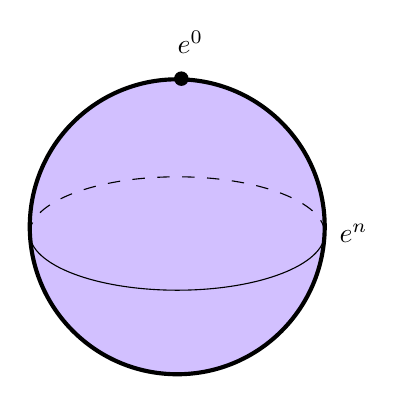
\begin{tikzpicture}[x=0.75pt,y=0.75pt,yscale=-1,xscale=1]
        \draw  [fill={rgb, 255:red, 210; green, 192; blue, 255 }  ,fill opacity=1 ][line width=1.5]  (217,132.06) .. controls (217,92.81) and (248.81,61) .. (288.06,61) .. controls (327.3,61) and (359.11,92.81) .. (359.11,132.06) .. controls (359.11,171.3) and (327.3,203.11) .. (288.06,203.11) .. controls (248.81,203.11) and (217,171.3) .. (217,132.06) -- cycle ; 
        \draw  [draw opacity=0][dash pattern={on 4.5pt off 4.5pt}] (217.01,135.79) .. controls (217,135.63) and (217,135.46) .. (217,135.3) .. controls (217,120.21) and (248.81,107.98) .. (288.06,107.98) .. controls (327.3,107.98) and (359.11,120.21) .. (359.11,135.3) .. controls (359.11,135.65) and (359.09,136) .. (359.06,136.35) -- (288.06,135.3) -- cycle ; \draw  [dash pattern={on 4.5pt off 4.5pt}] (217.01,135.79) .. controls (217,135.63) and (217,135.46) .. (217,135.3) .. controls (217,120.21) and (248.81,107.98) .. (288.06,107.98) .. controls (327.3,107.98) and (359.11,120.21) .. (359.11,135.3) .. controls (359.11,135.65) and (359.09,136) .. (359.06,136.35) ;  
        \draw  [draw opacity=0] (359.1,134.8) .. controls (359.11,134.97) and (359.11,135.13) .. (359.11,135.3) .. controls (359.11,150.39) and (327.3,162.62) .. (288.06,162.62) .. controls (248.81,162.62) and (217,150.39) .. (217,135.3) .. controls (217,134.94) and (217.02,134.59) .. (217.05,134.24) -- (288.06,135.3) -- cycle ; \draw   (359.1,134.8) .. controls (359.11,134.97) and (359.11,135.13) .. (359.11,135.3) .. controls (359.11,150.39) and (327.3,162.62) .. (288.06,162.62) .. controls (248.81,162.62) and (217,150.39) .. (217,135.3) .. controls (217,134.94) and (217.02,134.59) .. (217.05,134.24) ;  
        \draw  [color={rgb, 255:red, 0; green, 0; blue, 0 }  ,draw opacity=1 ][line width=5.25] [line join = round][line cap = round] (290.04,60.69) .. controls (290.04,60.69) and (290.04,60.69) .. (290.04,60.69) ;
        \draw (365,129.4) node [anchor=north west][inner sep=0.75pt]    {$e^{n}$};
        \draw (287,36.4) node [anchor=north west][inner sep=0.75pt]    {$e^{0}$};
    \end{tikzpicture}\]
\end{example}
\begin{proposition}
    令 $(X,\mathcal{E})$ 为一个 CW 复形, 以及 $\mathcal{E} = \coprod \mathcal{E}^n$, 其中 $\mathcal{E}^n$ 为 $n$ 维胞腔构成的集合, 记 $\Phi_n = \coprod_{e\in \mathcal{E}^n}\Phi_e$.
    则图表
    \[\begin{tikzcd}
	{\coprod_{e\in\mathcal{E}^n}S^{n-1}} & {X^{n-1}} \\
	{\coprod_{e\in\mathcal{E}^n}\mathbb{D}^n} & {X^n}
	\arrow["{\partial \Phi^n }", from=1-1, to=1-2]
	\arrow[hook, from=1-1, to=2-1]
	\arrow[from=1-2, to=2-2]
	\arrow["{\Phi^n}", from=2-1, to=2-2]
    \end{tikzcd}\]
    为推出图表.
    特别地, $X^n$ 由在 $X^{n-1}$ 上粘接 $X$ 的 $n$ 维胞腔得到.
\end{proposition}
\begin{proof}
    由 $X^{n-1}$ 为 $X^n$ 的闭子空间以及弱拓扑立刻得到.
\end{proof}
\section{CW-复形的拓扑性质}

\section{CW-复形的同伦性质}